\documentclass[tikz,border=8pt]{standalone}
\usepackage{sansmath}
\usetikzlibrary{calc,arrows.meta,positioning}

\begin{document}
\sansmath

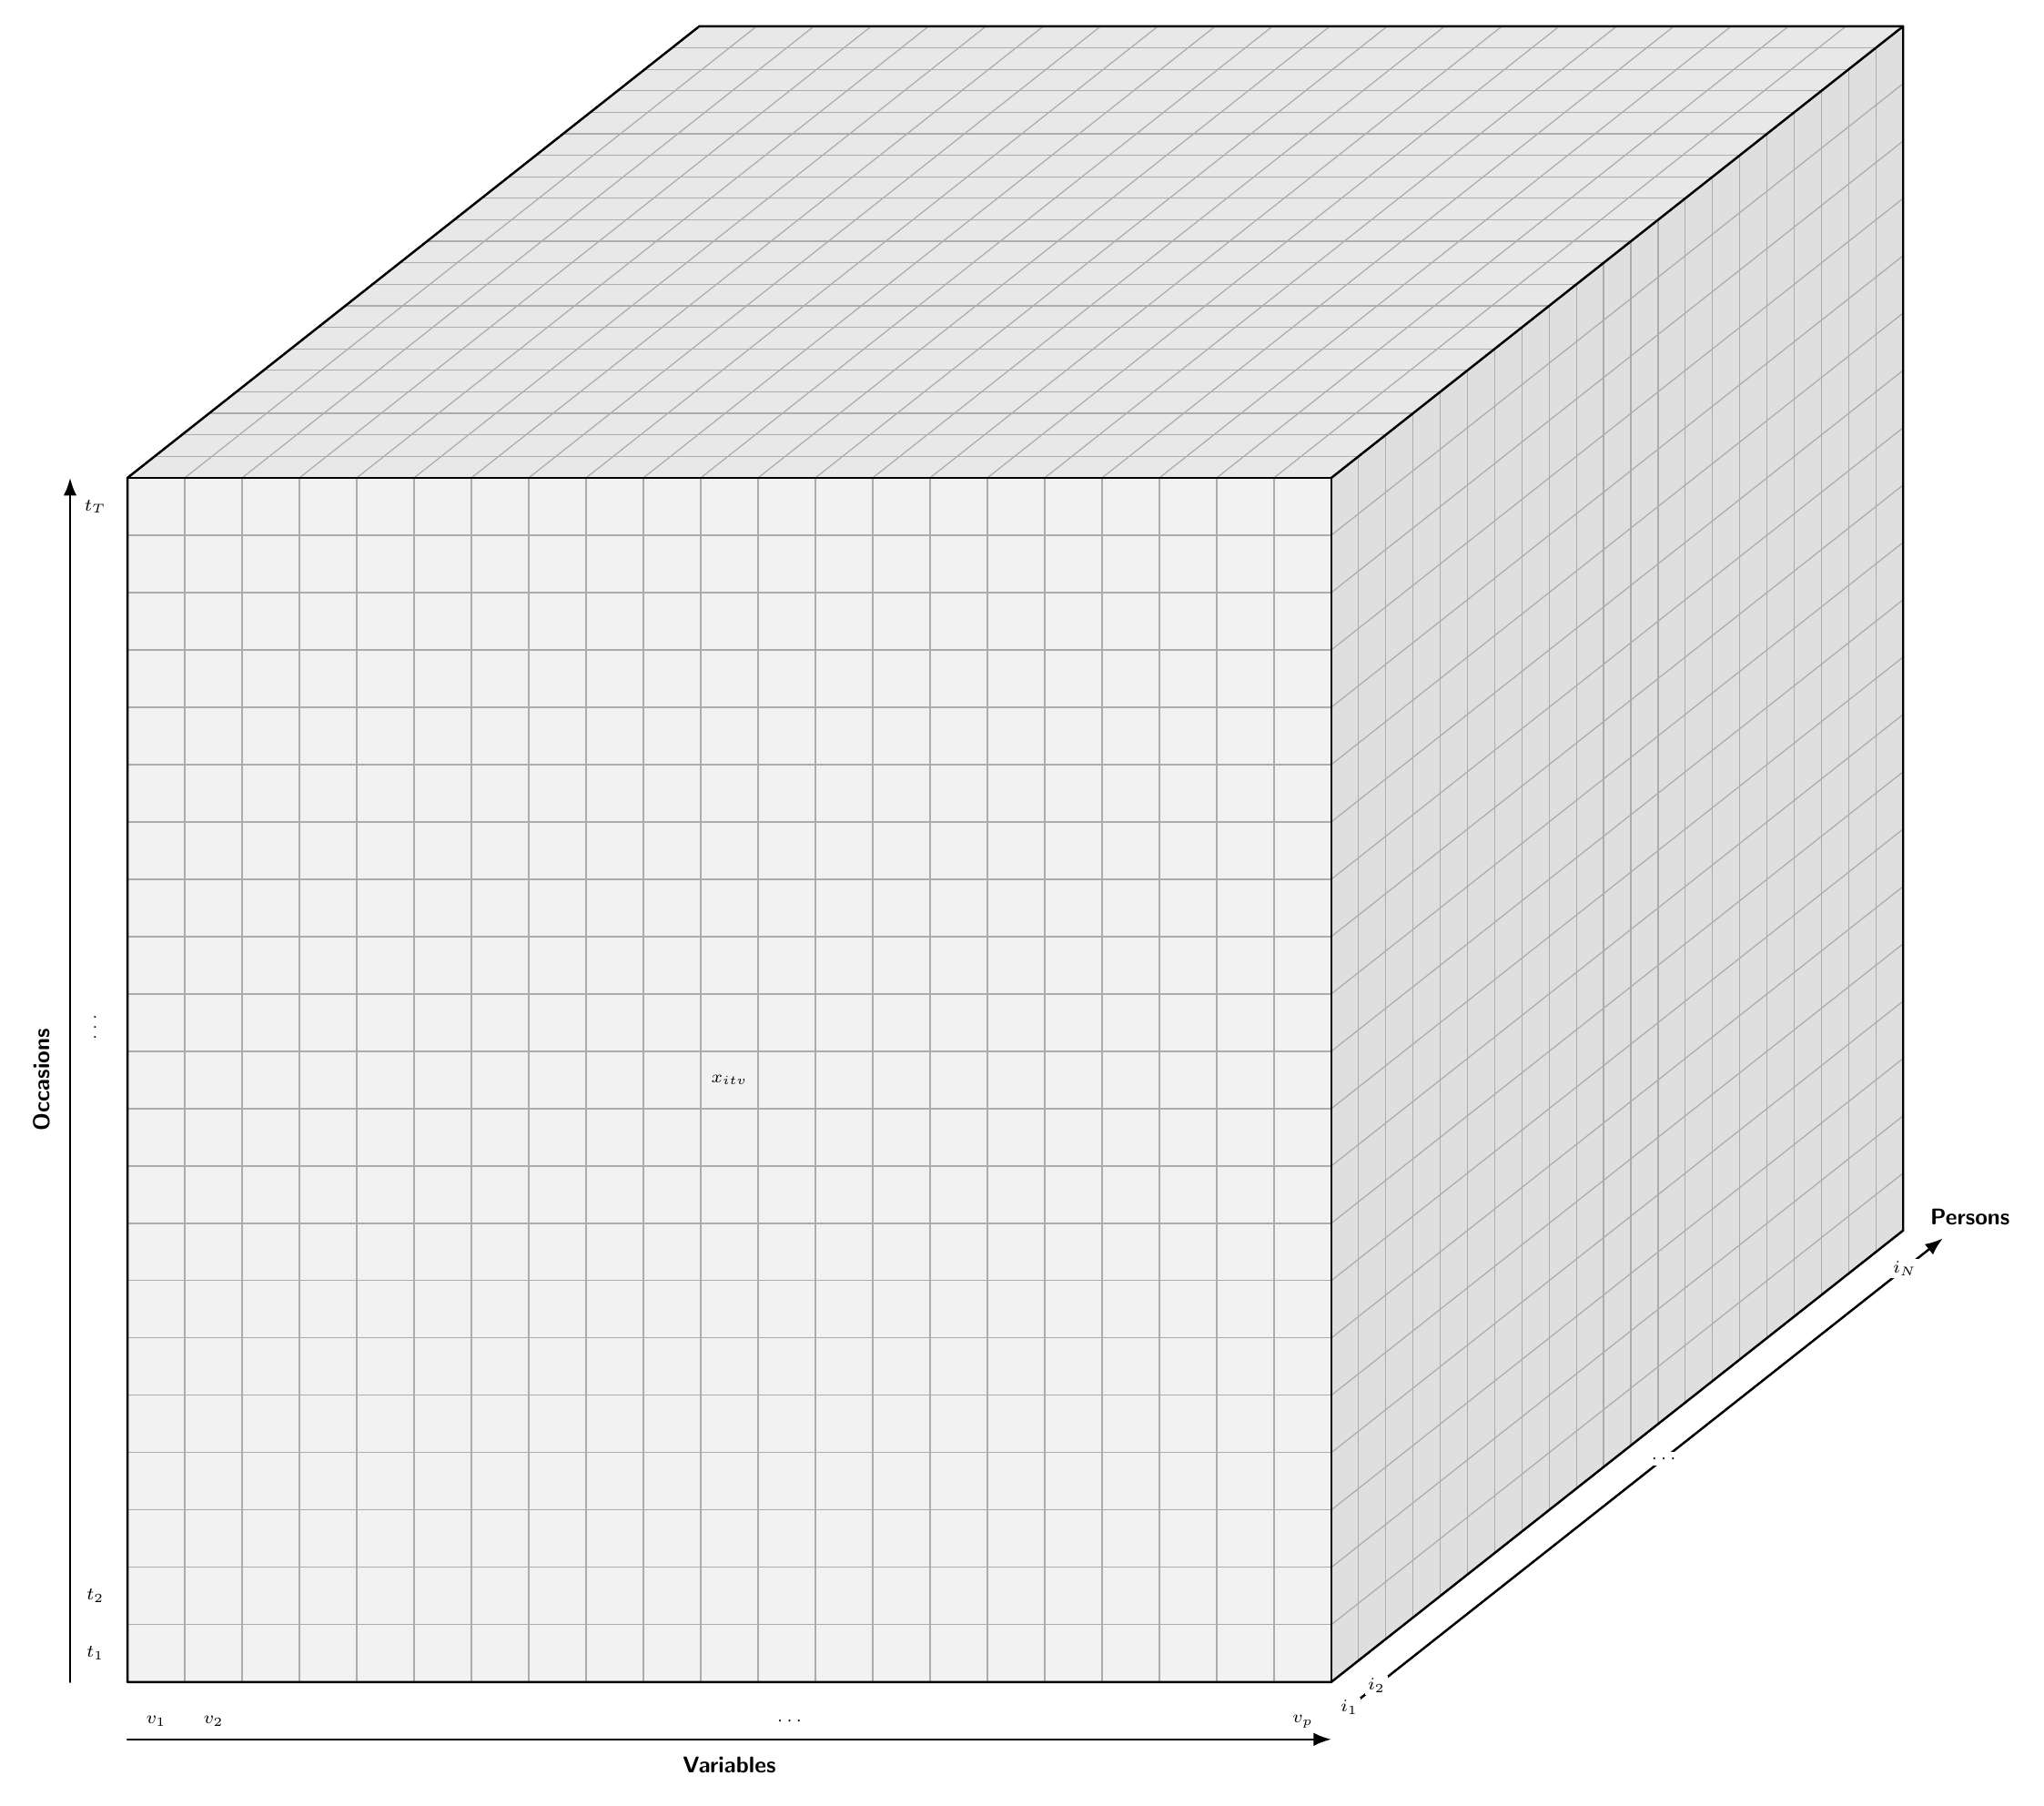
\begin{tikzpicture}[
		line join=round,
		line cap=round,
		font=\sffamily,
		>=Latex,
		axis/.style={->, line width=0.9pt},
		gridline/.style={gray!65, line width=0.45pt},
		outline/.style={black, line width=0.9pt},
		lab/.style={font=\sffamily\small},
		ticklab/.style={font=\sffamily\scriptsize, fill=white, inner sep=1pt},
		frontlab/.style={font=\sffamily\scriptsize, fill=gray!10, inner sep=1pt}
	]
	
	% Parameters
	\def\Nx{21} % variables
	\def\Ny{21} % occasions
	\def\Nz{21} % persons
	\def\a{0.8}
	\def\dx{0.38}
	\def\dy{0.30}
	
	\pgfmathsetmacro{\W}{\Nx*\a}
	\pgfmathsetmacro{\H}{\Ny*\a}
	\pgfmathsetmacro{\Dxx}{\Nz*\dx}
	\pgfmathsetmacro{\Dyy}{\Nz*\dy}
	
	% Adaptive tick positions
	\pgfmathsetmacro{\VarMid}{0.55*\Nx}
	\pgfmathsetmacro{\OccMid}{0.55*\Ny}
	\pgfmathsetmacro{\PerMid}{0.55*\Nz}
	
	% Persons axis placement controls
	\pgfmathsetmacro{\PersonAxisOffsetX}{0.25}
	\pgfmathsetmacro{\PersonAxisOffsetY}{-0.35}
	\pgfmathsetmacro{\PersonAxisExtra}{0.8}
	\pgfmathsetmacro{\PersonLabelGap}{1.0}
	
	% Precomputed persons-axis coordinates
	\pgfmathsetmacro{\PersonAxisStartX}{\W + \PersonAxisOffsetX}
	\pgfmathsetmacro{\PersonAxisStartY}{\PersonAxisOffsetY}
	\pgfmathsetmacro{\PersonAxisEndX}{\W + \PersonAxisOffsetX + (\Nz + \PersonAxisExtra)*\dx}
	\pgfmathsetmacro{\PersonAxisEndY}{\PersonAxisOffsetY + (\Nz + \PersonAxisExtra)*\dy}
	\pgfmathsetmacro{\PersonLabelX}{\W + \PersonAxisOffsetX + (\Nz + \PersonAxisExtra + \PersonLabelGap)*\dx}
	\pgfmathsetmacro{\PersonLabelY}{\PersonAxisOffsetY + (\Nz + \PersonAxisExtra + \PersonLabelGap)*\dy}
	
	% Precomputed tick-label coordinates
	\pgfmathsetmacro{\VarLastX}{(\Nx - 0.5)*\a}
	\pgfmathsetmacro{\OccLastY}{(\Ny - 0.5)*\a}
	\pgfmathsetmacro{\PerLastX}{\W + \PersonAxisOffsetX + (\Nz - 0.6)*\dx}
	\pgfmathsetmacro{\PerLastY}{\PersonAxisOffsetY + (\Nz - 0.6)*\dy}
	\pgfmathsetmacro{\PerMidX}{\W + \PersonAxisOffsetX + \PerMid*\dx}
	\pgfmathsetmacro{\PerMidY}{\PersonAxisOffsetY + \PerMid*\dy}
	\pgfmathsetmacro{\PerSecondX}{\W + \PersonAxisOffsetX + \dx}
	\pgfmathsetmacro{\PerSecondY}{\PersonAxisOffsetY + \dy}
	
	% Faces
	\fill[gray!10] (0,0) rectangle (\W,\H);
	\fill[gray!18] (0,\H) -- (\W,\H) -- (\W+\Dxx,\H+\Dyy) -- (\Dxx,\H+\Dyy) -- cycle;
	\fill[gray!25] (\W,0) -- (\W,\H) -- (\W+\Dxx,\H+\Dyy) -- (\W+\Dxx,\Dyy) -- cycle;
	
	% Front grid
	\foreach \i in {0,...,\Nx} {
		\draw[gridline] (\i*\a,0) -- (\i*\a,\H);
	}
	\foreach \j in {0,...,\Ny} {
		\draw[gridline] (0,\j*\a) -- (\W,\j*\a);
	}
	
	% Top grid
	\foreach \i in {0,...,\Nx} {
		\draw[gridline] (\i*\a,\H) -- (\i*\a+\Dxx,\H+\Dyy);
	}
	\foreach \k in {0,...,\Nz} {
		\draw[gridline] (\k*\dx,\H+\k*\dy) -- (\W+\k*\dx,\H+\k*\dy);
	}
	
	% Side grid
	\foreach \j in {0,...,\Ny} {
		\draw[gridline] (\W,\j*\a) -- (\W+\Dxx,\j*\a+\Dyy);
	}
	\foreach \k in {0,...,\Nz} {
		\draw[gridline] (\W+\k*\dx,\k*\dy) -- (\W+\k*\dx,\H+\k*\dy);
	}
	
	% Outer outline
	\draw[outline]
	(0,0) -- (\W,0) -- (\W+\Dxx,\Dyy) -- (\W+\Dxx,\H+\Dyy)
	-- (\Dxx,\H+\Dyy) -- (0,\H) -- cycle;
	\draw[outline] (\W,0) -- (\W,\H) -- (0,\H);
	\draw[outline] (\W,\H) -- (\W+\Dxx,\H+\Dyy);
	
	% External axes
	\draw[axis] (0,-0.8) -- (\W,-0.8);
	\node[lab] at (\W/2,-1.15) {\bfseries Variables};
	
	\draw[axis] (-0.8,0) -- (-0.8,\H);
	\node[lab, rotate=90] at (-1.2,\H/2) {\bfseries Occasions};
	
	\draw[axis] (\PersonAxisStartX,\PersonAxisStartY) -- (\PersonAxisEndX,\PersonAxisEndY);
	\node[lab] at (\PersonLabelX,\PersonLabelY) {\bfseries Persons};
	
	% Tick labels for variables
	\node[ticklab] at (0.5*\a,-0.55) {$v_1$};
	\node[ticklab] at (1.5*\a,-0.55) {$v_2$};
	\node[ticklab] at (\VarMid*\a,-0.55) {$\cdots$};
	\node[ticklab] at (\VarLastX,-0.55) {$v_p$};
	
	% Tick labels for occasions
	\node[ticklab] at (-0.45,0.5*\a) {$t_1$};
	\node[ticklab] at (-0.45,1.5*\a) {$t_2$};
	\node[ticklab] at (-0.45,\OccMid*\a) {$\vdots$};
	\node[ticklab] at (-0.45,\OccLastY) {$t_T$};
	
	% Tick labels for persons
	\node[ticklab] at (\PersonAxisStartX,\PersonAxisStartY) {$i_1$};
	\node[ticklab] at (\PerSecondX,\PerSecondY) {$i_2$};
	\node[ticklab] at (\PerMidX,\PerMidY) {$\cdots$};
	\node[ticklab] at (\PerLastX,\PerLastY) {$i_N$};
	
	% Example observation label
	\node[frontlab] at (0.5*\W,0.5*\H) {$x_{itv}$};
	
\end{tikzpicture}

\end{document}